\documentclass[12pt]{article}

\usepackage{sbc-template}
\usepackage{graphicx,url}
\usepackage[utf8]{inputenc}
\usepackage[portuges]{babel}
     
\sloppy

\title{EASYCODE: UM AMBIENTE DE TECNOLOGIAS DE APOIO PARA O ENSINO DE LÓGICA DE PROGRAMAÇÃO}

\author{Daniela F. Feitosa \inst{1}, Eduardo N. B. Neves \inst{1}, Emmerson S. R. Silva \inst{1}, Jucimar B. Souza \inst{1}}

\address{Instituto Federal de Educação, Ciência e Tecnologia do Amazonas \\ Campus Manaus Centro (IFAM-CMC)
  \email{\{danielaferreira1133, eddunic,  emmsr2004, jucibs\}@gmail.com}
}

\begin{document} 

\maketitle

\begin{abstract}
This article presents the scientific contribution aimed at the EasyCode software, developed by IFAM-CMC students in 2017, aiming to adapt it to students who have difficulty applying the programming logic of the imperative paradigm in the resolution of computational problems. The application is being developed in the web platform and will consist of visual programming based on programming blocks, flowcharts and application of the cognitive domain of the Revised Bloom Taxonomy (ANDERSON et al., 2001) in a future gamification in order to stimulate the assimilation of concepts of logic. The technologies that will used in the teaching-learning process will allow programming concepts to be understood in a playful way.

\end{abstract}
     
\begin{resumo}
Este artigo apresenta a contribuição científica objetivada para o software EasyCode, desenvolvido por alunos do IFAM-CMC em 2017, visando adequá-lo aos estudantes que têm dificuldade em aplicar a lógica de programação do paradigma imperativo na resolução de problemas computacionais. A aplicação está sendo desenvolvida na plataforma web e consistirá na programação visual com base em blocos de programação, fluxogramas e na aplicação do domínio cognitivo da Taxonomia de Bloom Revisada (ANDERSON et al., 2001) em uma futura gamificação a fim de estimular a assimilação dos conceitos da lógica. As tecnologias ao serem empregadas no processo de ensino-aprendizagem permitirão que conceitos da programação sejam compreendidos de maneira lúdica.
\end{resumo}

\section{Introdução}
As dificuldades que inviabilizam a compreensão da programação variam desde a abordagem utilizada para o ensino até o problema na natureza cognitiva do aluno. Segundo Gomes \textit{et al.} (2008), dentre os possíveis fatores deste problema destacam-se o elevado nível de abstração da programação e a falta de motivação do próprio aluno. 
\\Em um estudo de caso baseado na Taxonomia de Bloom e no Scratch, realizado por Araújo \textit{et al.} (2013), percebeu-se a necessidade de incentivo ao aprendizado e do uso de outros recursos visuais como base metodológica. Portanto, modificações na abordagem utilizada durante as aulas de lógica podem torná-las mais interativas e despertarem gradativamente o interesse do aluno, apesar das possíveis dificuldades enfrentadas (SILVA \textit{et al.}, 2017).
\\O \textit{software} EasyCode desenvolvido por SILVA \textit{et al.} (2017) dispõe de um ambiente de programação visual baseado em blocos e desenvolvido em Java Swing para ser empregado no aprendizado de lógica de programação, veja Figura 1. Este \textit{software} apresenta limitações, como: só é executado localmente em uma máquina (requer \textit{download} do programa), converte o algoritmo apenas para a linguagem C e, além da má organização dos blocos, apresenta uma interface confusa e pouco atrativa. Objetiva-se neste trabalho, uma nova fase de desenvolvimento voltada à \textit{web} com conversão para multilinguagens e com a implementação de novas tecnologias que ampliem as funcionalidades para o público-alvo.

\section{Metodologia} 
Utilizar-se-á o domínio cognitivo da Taxonomia de Bloom Revisada que consiste nas categorias lembrar, entender, aplicar, analisar, avaliar e criar (FERRAZ \textit{et al.}, 2010) para que ocorra a integração de abordagens de ensino que se adequem aos tipos de aprendizagem. Esta será a base metodológica para a gamificação que será implementada no \textit{software} EasyCode, que contará com uma sessão de desafios onde o discente poderá revisar o conteúdo de lógica de programação imperativa (inicialmente as estruturas lógicas), codificar e gerar fluxogramas ou a montagem de blocos, testar os códigos produzidos e avaliá-los, além de produzir e planejar técnicas de resoluções diversas.
\\Ademais, a taxonomia em conjunto com pesquisas quanti-qualitativas serão aplicadas para alunos do primeiro ano do ensino médio técnico em informática no IFAM-CMC para avaliar o nível de desenvoltura na resolução de problemas computacionais a partir do \textit{software} EasyCode.
\\Como ferramentas de desenvolvimento do \textit{website} estão sendo aplicados os \textit{frameworks} Maven, Hibernate e Bootstrap; as bibliotecas JQuery e Blocky; o padrão de arquitetura MVC; a metodologia ágil SCRUM; o controle de versão pelo GitHub; e a API JDBC. No \textit{front-end}, além do Bootstrap, utiliza-se a linguagem HTML5, JavaScript e as folhas de estilo em CSS3. O padrão XML está voltado para armazenar os blocos de programação, os processos de fluxogramas e o código-fonte gerado pela interação entre usuário e \textit{software}. 


\section{Resultados Parciais e Discussão}
	\begin{figure}[h]
		\centering
		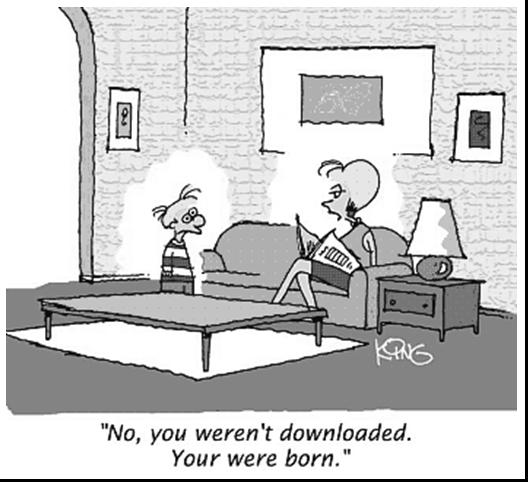
\includegraphics[scale=0.2]{fig1.jpg}
		\caption{Uma típica figura.}
		\label{fig1}
	\end{figure}

\section{Considerações Parciais}
O EasyCode é um ambiente que proporciona os recursos da programação e da robótica para permitir que alunos com dificuldades em compreender a lógica de programação possam aprender a programar de maneira simples e prática. Espera-se que as mudanças propostas colaborem com o processo de ensino-aprendizagem, por exemplo, permitindo que professores possam demonstrar de forma mais lúdica conceitos da programação e também que ocorra a adequação da abordagem de ensino aos tipos de aprendizagem. 
\\A visualização por meio de fluxogramas dos passos para se construir o algoritmo permitirá o entendimento da aplicação da codificação de maneira simples. A implantação da conversão entre multilinguagens de programação e da biblioteca Blocky da Google permitirá que a ferramenta se torne mais atrativa para qualquer estudante.
\\Os alvitres para a continuidade do projeto em questão possuem a intenção de aumentar a usabilidade do referido por meio da eficácia do planejado. Através dos meios acessíveis impostos, pretende-se aumentar o alcance de uso do software por intermédio da implementação em plataforma \textit{web}. 

\bibliographystyle{sbc}
\bibliography{ArtigoEC}

\end{document}